
\chapter{Methods\label{cha:methods}}


\section{Experimental data aqcuisition}\label{sec:expdata}
\noindent
\indent The model implemented in this project aims to explain the mechanism of serotonin's effects during anaesthesia. Particularly, the model is tailored to the recording procedure and findings that were obtained in an experiment designed and conducted by Dr. Guido Meijer at the Champalimaud Foundation in Lisbon, Portugal. In this experiment, neural activity in several brain regions was measured using Neuropixels (electrodes measuring electrophysiological activity), after transient stimulation of the serotonergic neurons in the DRN. For precise and local stimulation, optogenetics \cite{deisseroth2015optogenetics} was used. The experiment was conducted on anaesthetized mice.\\
\indent The following areas were recorded and replicated in the model: superior colliculus (SC), midbrain reticular nucleus (MRN), secondary motor cortex (M2), medial prefrontal cortex (mPFC), 
orbitofrontal cortex (OFC), piriform cortex (PIR), striatum (STR), Amygdala (Amyg), retrosplenial cortex (RSP),  visual cortex (VIS), hippocampus (Hipp), striatum (Str), olfactory cortex (OLF), and piriform cortex (Pir).

\section{Model structure}

\noindent
\indent The model implemented in this project is a bistable firing rate model, consisting of multiple local circuits that all-to-all connected form a global network. The local circuits represent the relevant brain areas from the experimental recordings. Serotonin stimulation is modelled by inducing a current to all regions, originating from the DRN. Furthermore, it includes connectivity data from the Allen Brain Atlas that define the connectivity between the regions in the model as well as the projection density from the DRN to the different regions.  

\subsection{Local circuit model \label{sec:lc}}
\noindent
\indent This section describes the local circuit model which is used to simulate the average firing rate in individual brain areas in the model. The local circuit model has to fulfil the condition that it is a dynamical firing rate model, which produces UP and DOWN states similar to the states that could be recorded during anaesthesia \cite{ruiz-mejiasSlowFastRhythms2011}. Therefore, we chose a model proposed by Jercog et al. \cite{jercogUPDOWNCorticalDynamics2017}, which is a simplistic model including one excitatory population $E$ and one inhibitory population $I$. Furthermore, it includes an adaptation module $a$, which simulates synaptic fatigue in pyramidal cells, as well as background noise which is introduced to the E and I population. There are projections implemented between both populations, as well as a self coupling mechanism. 

The local circuit model follows three main equations, as defined in Jercog et al. \cite{jercogUPDOWNCorticalDynamics2017}, which describe the change of the populations $E$ and $I$ firing rate $r$ (see Equation \ref{eq:1} and \ref{eq:2}), as well as the strength of adaptation $a$ (see Equation \ref{eq:3}) over time, where $\tau_E, \tau_I$ and $\tau_a$ are time constants.

\begin{equation}\label{eq:1}
    \tau_E \frac{dr_E}{dt} = -r_E(t) + \varphi_E (J_{EE}r_E(t) - J_{EI}r_I(t)-a(t)+\sigma\xi_E(t))
\end{equation}

\begin{equation}\label{eq:2}
    \tau_I \frac{dr_I}{dt} = -r_I(t) + \varphi_I (J_{IE}r_E(t) - J_{II}r_I(t)+\sigma\xi_I(t))
\end{equation}

\begin{equation}\label{eq:3}
    \tau_a \frac{da}{dt} = -a(t) + \beta r_E(t)
\end{equation}

The frequency of UP and DOWN state changes is defined by $\frac{1}{\tau_a}$, so the original value of ${\tau_a=500ms}$ generates states in the frequency of around 2Hz. Analyses of the experimental data in the mouse revealed that the frequency of state change is 0.5-1Hz, therefore a value of $\tau_a=1500ms$ was chosen and the other time constants were scaled accordingly, so that for the final implementation it yields that $\tau_E=30ms$ and $\tau_I=6ms$. 
\\
The variable $J$ defines the local coupling strength for the E and I population, which is $J_EI = 5$, $J_EE = 1$, $J_EE = 10$, and $J_EE = 0.5$ (the first letter indicating the target population).  
\\
\\
\indent To model the noise of the system, which is introduced as a background noise to both populations, two Ornstein-Uhlenbeck processes are implemented, with a mean of zero and a standard deviation of $\sigma=3.5$. 
\\
The functions $\varphi_E$ and $\varphi_I$ are called the transfer functions, which determine the reaction of the population to incoming currents, through self coupling, projections coming from other populations, or/and background noise. The equation is a threshold-linear function, with a threshold that defines the start of the linear part of the equation. If the input does not reach the threshold, the activation of the regarding population is set to zero. 

\begin{equation}\label{eq:4}
    \varphi_X(x) = g_X[x-\theta_X]_+\qquad,X=\{E,I\}
\end{equation}

The threshold that has to be reached until the population reacts to incoming input is described by $\theta$. The value that I used for the implementation of brain regions that show UP and DOWN states is $\theta_E = 6$ and $\theta_I = 25$. The choice of those parameters is explained in the following section.
\\
In case the input reaches the threshold level, the slope $g$ determines the output. The $g$ controls how sensitive the population reacts to input. A higher $g$ will lead to a stronger output than a lower $g$. The original values are $g_E = 1Hz$ and $g_I = 4Hz$, which will be manipulated later on, in order to reach firing rates that are more similar to the experimentally measured firing rates. 
\\

\noindent\textbf{UP and DOWN state dynamics}
\\
\indent Several components of the model play a role to generate the UP-DOWN dynamics. Most importantly, the system requires bistability, meaning that the model has two stable states of activity, which are called stable attractor points. When one of those points is reached, the network stays at that rate of activity if there is no perturbing signal from the outside reaching the network. The first attractor point represents the DOWN state, in which no firing rate is observed. The second attractor point represents the UP state, with an average firing rate that depends on the setting of local connectivity parameters (self coupling and coupling between E and I). The bistability of the local circuit is reached by the coupling between E and I population and the way the transfer functions are implemented. To find the two attractor points of the system, refer to the nullclines of $r_E(t)$ and $r_I(t)$. Equation \ref{eq:4} and \ref{eq:5} describes $r_E(t)$ and $r_I(t)$, and when solving the equation with setting $r_E=0$ and $r_I=0$, it yields the nullcline of each population. Under specific conditions the nullclines intersect at two points, which are the two attractor points in which both firing rates stay the same.

\begin{equation}\label{eq:5}
    r_E = g_E[J_EEr_E-J_EIrI-a-\theta_E]_+
\end{equation}

\begin{equation} %\label{eq:5}
    r_I = g_I[J_IEr_E-J_IIrI-\theta_I]_+
\end{equation}

Where the two nullclines intersect depends on the threshold $\theta$ of both populations, since it defines the start of the incline of the linear function. If $\theta_E < \theta_I$, the nullcline of $r_E$ has time to incline linearly, whereas the nullcline of $r_I$ starts rising from zero only later on (see Figure \ref{fig:phase_diagram1} A). The fact that $g_E < g_I$, allows the nullclines to intersect and therefore allowing the stable attractor point for the UP state arise (see Figure \ref{fig:phase_diagram2} A). 



\begin{figure}[h]
    \centering
    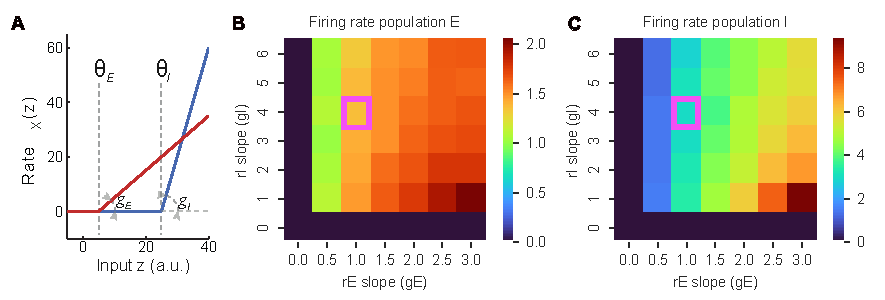
\includegraphics{img/Methods/Figure2_1.pdf}
    \caption[Nullclines of rE and rI and the effect of their slope on E and I firing rates]{A) Nullclines of rE and rI (taken from Jercog et al. \cite{jercogUPDOWNCorticalDynamics2017}). The effect of the nullclines' slope on the B) E and C) I populations' firing rate. The purple square indicates the default parameter setting.}
    \label{fig:phase_diagram1}
\end{figure}


Adaptation and the fluctuating noise in both populations can initiate the change between the two attractor points of the system. The threshold of the excitatory population $\theta_E$ and the adaptation strength $\beta$ are two parameters that determine the transitions between one state to the other. Figure \ref{fig:phase_diagram2} C) visualises the change of UP and DOWN state frequencies in a phase diagram of the parameters $\beta$ and $\theta_E$.
\\
\indent The circuit dynamics can be described with a limit cycle regime with oscillatory pattern of $\frac{1}{tau_A} Hz$. The originally defined time constants produce UP and DOWN activity with the frequency of 2 Hz. Since the electrophysiological recordings from the mouse brain showed that the UP and DOWN states have a frequency of 0.5-1 Hz, all time constants in the model were multiplied by 3, which leads to lower frequencies (see Figure \ref{fig:phase_diagram2} C).
\\
\begin{figure}[h]
    \centering
    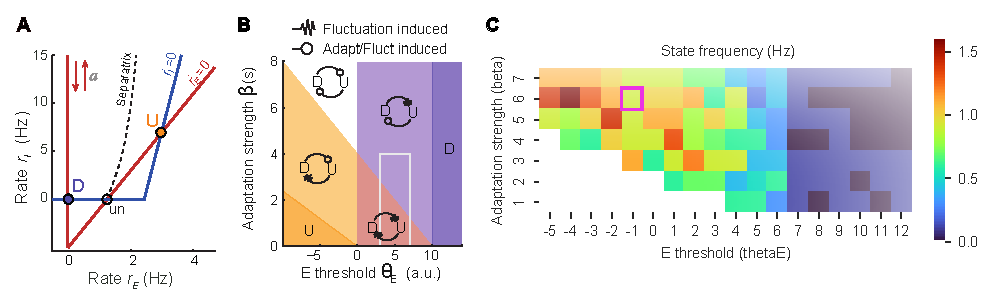
\includegraphics[width=1\textwidth]{img/Methods/Figure2_2.pdf}
    \caption[The role of the excitatory firing threshold and the adaptation strength in the UP-DOWN dynamics]{The role of the excitatory firing threshold and the adaptation strength in the UP-DOWN dynamics. A) Adapted from Jercog et al. \cite{jercogUPDOWNCorticalDynamics2017}, showing the two attractor points (U and D for UP and DOWN state) where the nullclines of rE and rI intersect. The current adaptation $\alpha$ value determines the position of the rE nullcline on the y-axis which can lead to the switch between the two attractor points. B) Taken from Jercog et al. \cite{jercogUPDOWNCorticalDynamics2017}, showing the phases in which the cuircuit switches between states with transitions induced by noise fluctuations or adaptation. C) Phase diagram showing the frequency of UP-DOWN states depending on the excitatory threshold and adaptation strength (using original time constant scaled by 3). Empty fields indicate absence of UP-DOWN states. The purple square indicates the setting for regions that show UP and DOWN states.}
    \label{fig:phase_diagram2}
\end{figure}
\subsection{Global circuit\label{sec:gc}}
\noindent
\indent By combining several local circuits, we implement a network of brain areas. The goal is to simulate the brain areas that were measured experimentally (see \ref{sec:expdata} for names of all simulated regions).


\subsection{Heterogeneity}
\noindent
\indent The brain regions that are modelled in this project are heterogeneous in terms of firing rate, and characteristics of UP and DOWN states. The electrophysiological measurements show that some regions only show UP states, whereas others show a clear UP-DOWN dynamic. The goal is to incorporate this behaviour in the network model. As we know from the local circuit model, the frequency of the UP and DOWN states can be modified by changing the adaptation strength $\beta$ and the threshold of the E population $\theta_E$. Areas that show UP-DOWN dynamics in the electrophysiological recordings in anaesthetised mice are cortical areas as well as the striatum. A value of $\beta = 6$ and $\theta_E = 4$ is set for those regions, since a strong adaptation value leads to reliable generation of UP and DOWN states. Areas that do not show DOWN states, are midbrain areas as well as the hippocampus. This behaviour is achieved by using a low adaptation value $\beta = 1$ and a slightly higher threshold for E $\theta_E = 5$. Regions that show more unclear UP-DOWN states in the electrophysiological data receive a parameter setting of a medium adaptation value $\beta = 3$ and $\theta_E = 5$.
\\
\indent Besides the state frequency, the average firing rate of the E and I populations in each area can be adapted to match the experimental data. The adjustment is realised by cautiously modifying the slope of each populations transfer function (the $g$ in Equation \ref{eq:4}). This modification of the firing rates in each of the local circuit models (brain areas) so that the average firing rate of the E and I population is slightly below the value measured in the mouse brain, since this value will increase later on due to the communication between the areas. The average firing rate values in the model therefore approximate the measured rates (+-5 spikes per seconds).  
\subsection{Connectivity\label{sec:abc}}
\noindent
\indent The Allen Brain Institute provides an atlas of the mouse brain, including the connectivity between brain regions. This allows for more realistic modelling of the global circuit, and the investigation of the question of how relevant (heterogeneous) projections are.
The Allen Brain Atlas can be accessed by using the API that is provided. The package \verb|allensdk| \cite{fulcherBenfulcherAllenSDKInitial2020} was used for this purpose. The Mouse Connectivity Atlas contains experiments about the projections between brain areas in Cre-modified and normal mice. In each experiment, the researchers injected a retrograde viral tracer into a brain structure. The brain areas that were downloaded from the Mouse Connectivity Atlas were chosen based on the areas identified in the recordings of the experimental study (Meijer et al., in preparation). The areas in the experimental study were defined in terms of the Beryl atlas, which is an atlas that is mapping brain structures with acronyms and parcellations slightly different from the Allen Brain Atlas. The regions defined in Beryl annotations were translated to the appropriate brain regions in the Allen atlas and grouped together to higher level areas. For each area, we obtained the projection density values to all relevant areas. Results from all experiments per region were averaged. Since some experiments do not show any projection values, a threshold of a projection density of 0.005 was applied for the experiment to be included. As a next step, the obtained values of the fine grained areas were grouped together into higher level brain areas that each represent one component of the network (see Figure \ref{fig:connectivity}).
\\
\begin{figure}[h]
    \centering
    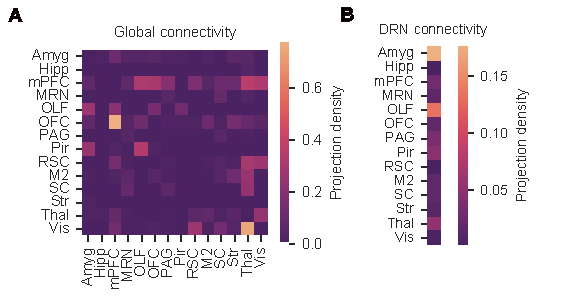
\includegraphics[width=0.8\textwidth]{img/Methods/figure1.pdf}
    \caption[Connectivity from the Allen Brain Atlas]{Connectivity from the Allen Brain Atlas. A) shows the long-range projections between areas (x-axis: target regions) and B) the serotonergic projections originating from the DRN.}
    \label{fig:connectivity}
\end{figure}

\indent Besides the connectivity values between the areas within the network, the serotonergic projections originating from the DRN are required to simulate the release of serotonin, since the DRN projects to some regions more than to others. For this, we used experiments in which selectively serotonergic projections are traced. Similar to the connectivity matrix, the results are grouped together into the areas that are relevant in the network model (see Figure \ref{fig:connectivity}). 
\\
\indent To introduce the connectivity data in the global network model, the projection density values $W^{xy}$ (projection to area $x$ from area $y$) are multiplied with the coupling strength $G$ between the inter-area projections. The input into population E of area $x$ can therefore be defined as $I^x_E$ from projections that originate from all other areas y (see Equation \ref{eq:8}). 

\begin{equation}\label{eq:8}
    I^x_E = G \sum_y W^{xy}
\end{equation}



\subsection{Modelling Serotonin Stimulation\label{sec:mss}}

\indent 

To simulate the inhibitory effect that serotonin seems to have on most brain areas during anaesthesia, a current that represents the input from serotonergic neurons originating from the DRN projecting to the isolated local circuits is introduced. Similar to the connectivity matrix for the inter-area long-range projections, the projections of the DRN are weighted depending on the projection density. Considering that the DRN projection densities to all areas $x$ are stored in a vector $\vec{D}$ the input current $I_{DRN}$ is defined as the following:


\begin{equation}\label{eq:9}
    I^x_{DRN}(t) = S\vec{D}_x u(t)
\end{equation}

The recorded neurons in the mouse brain react to serotonin release in a trajectory in which there is a peak modulation observed after 0.5 seconds and a decay of this effect until it returns to the original state before optogenetic stimulation after 3 seconds. The time curve of this trajectory, here defined as $u(t)$ (see Figure \ref{fig:serotonin_release}) is multiplied with the parameter for serotonin stimulation strength $S$ and is therefore simulating the gradual serotonin release and delayed decay. The stimulation is applied for 1 second, in an inter-trial interval of 3-6 seconds, simulating transient optogenetic stimulation, mimicking the experimental procedure.
\\
\begin{figure}[h]
    \centering
    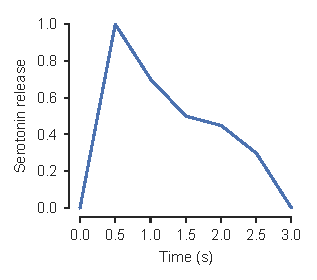
\includegraphics[width=0.4\textwidth]{img/Methods/serotonin_trajectory.pdf}
    \caption[Serotonin release trajectory]{Serotonin release trajectory $u(t)$. Estimated based on experimental data. A serotonin release of 1 indicates the full possible capacity of its release.}
    \label{fig:serotonin_release} 
\end{figure}

Now, the target of the serotonin stimulation $I_{DRN}$ in the model is considered. The transition from an UP towards a DOWN state is influenced by the threshold $\theta_E$ and the E populations' capability of reaching this threshold. Lowering the input to the E population makes it more difficult for the E population to reach $\theta_E$. At the same time, as the adaptation towards E increases, it makes it even harder to reach the threshold and the system can eventually not stay in an UP state anymore, and therefore transitions into a DOWN state. By introducing an inhibitory current to the E population (subtracting  $I_{DRN}$ from $r_E$), it becomes harder to cross the threshold and it is more likely that the system eventually transitions into a DOWN state, which is exactly the effect that serotonin seems to have on the brain network. 
\\

\begin{figure}[h]
    \centering
    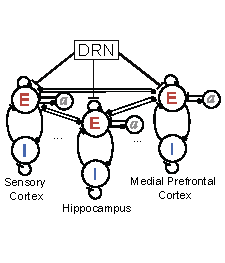
\includegraphics[width=0.4\textwidth]{img/Methods/GlobalModel.pdf}
    \caption[Global network model]{Global network model. The implemented model comprises 14 areas (3 example regions are displayed), which are interconnected.}
    \label{fig:connect} 
\end{figure}

The described global model is extending the local circuit model proposed by Jercog et al. \cite{jercogUPDOWNCorticalDynamics2017}. The dynamics of the global model are formulated in Equation \ref{eq:6} (for the E population) and Equation \ref{eq:7} (for the I population). The formula for the adaptation remains as described in Equation \ref{eq:3}

\begin{equation}\label{eq:6}
\tau \frac{dr_E}{dt} = - r_E(t) J_{EE} r_E(t) - J_{EI} r_I(t) - r_A(t) + \theta_E + \sigma \xi_X(t) + I_E - I_{DRN}
\end{equation}

\begin{equation}\label{eq:7}
        \tau \frac{dr_I}{dt} = -r_I(t) J_{II} r_I(t) - J_{IE} r_E(t) + \theta_I + \sigma \xi_X(t) \\[20pt]
\end{equation}

\section{Model modifications}
\noindent
\indent To examine which components of the model are crucial for the replication of serotonin's effect, a subset of the simulations are run with a slightly modified model. 
\subsection{Modified connectivity}
\noindent
\indent The goal is to shine light on the role of connectivity in the brain on the effect of serotonin, and therefore understand the importance of communication between the different areas. For this purpose, two aspects are examined: 1) the strength, and 2) the heterogeneity of the coupling. The coupling strength was modified by changing the value of $G$. To test the relevance of heterogeneous coupling, the connectivity matrix was replaced by a unique value for all brain areas. To ensure that this homogeneous connectivity is not too strong or too weak, the value is calculated from the mean of the connectivity matrix, so that $W$ is replaced by \(\bar{W} = \frac{1}{n} \sum W\).

\subsection{Modulating the mechanism of modelling serotonin}
\noindent
\indent Intuitively, adding a current to the I populations rate should lead to the same effect, as it shifts the I nullcline to the left, such that the attractor point representing the UP state (intersection of the two nullclines) eventually disappears and the system would transition into a DOWN state. 
To validate the assumption and determine if stimulation can induce DOWN states through alternative means, simulations in which population I is targeted by an excitatory current were run. This is achieved by adding 
$I_{DRN}$ to $r_I$ instead of subtracting $I_{DRN}$ from $r_E$.
\\
\indent Given the potential for unexpected results in exploring the different mechanisms of serotonin stimulation, additional simulations were performed by targeting the E population with an excitatory current (reverting the sign of $I_{DRN}$ in Equation \ref{eq:6}) and the I population with an inhibitory current (subtracting $I_{DRN}$ from $r_I$). These simulations aim to determine if these mechanisms would also lead to a comparable effect and to evaluate the significance of the chosen approach for modelling serotonin stimulation in achieving the observed effects in the experimental data.

\section{Analysis methodologies}

\subsubsection{Hidden Markov Model for state classification\label{sec:hmm}}
\noindent
\indent To analyse the UP and DOWN states in the simulated activity, a Hidden Markov Model (HMM) was applied. We used the package \verb|ssm| developed by Linderman et al. \cite{Linderman_SSM_Bayesian_Learning_2020}, which implements state classification with HMMs using Bayesian inference. To classify the states using HMMs, first, a HMM model has to be defined, and the number of possible states has to be specified. Then, the HMM is fit to the firing rate data. Here, we used the I population's firing rate, since it is easier to classify based on its high firing rate relative to the E population's firing rate. It is now possible to predict the most likely state for every time step. Based on the HMM state classification, analyses of the probability of a certain state at a given time are possible.

\subsection{Synchrony in the global network model}\label{cha:brunel}
\noindent
\indent Previous evidence showed that inter-area communication introduces synchrony within a network \cite{varelaBrainwebPhaseSynchronization2001, holcmanEmergenceStatesCortical2006}. This might also be the case of the UP-DOWN dynamics that occur in each area. For example, if an UP state is induced in one area, the elevated firing rate is propagated to the E population of the other areas, increasing the chance of a simultaneous transition into an UP state in the targeted areas. To measure the synchrony of the areas in the network, we computed the parameter $\chi(N)$ proposed by Brunel \cite{brunelCommunicatedPaulTiesinga2006} (see Equation \ref{eq:brunel1} and \ref{eq:brunel2}). The idea behind the formula is to take the variance
oan each isolated area and compare it to the variance of the entire network. $N$ denotes the number of local areas in the network, and r is the I population's firing rate.  

\begin{equation}\label{eq:brunel1}
    \sigma^2_r = \langle [r(t)]^2  \rangle_t - [
 \langle r(t) \rangle_t]^2 
\end{equation}

\begin{equation}\label{eq:brunel2}
    \chi(N) = \sqrt{\frac{\sigma^2_x}{\frac{1}{N}\sum^N_(i=1)\sigma^2_{r_i}}}
\end{equation}

This formula will provide us with information about the synchrony of every region compared to the global synchrony.
